\documentclass[13pt]{article}

\RequirePackage{latexsym}
\RequirePackage{amsmath}
\RequirePackage[many]{tcolorbox}
\RequirePackage{amssymb}
\RequirePackage{bm}
\RequirePackage{dsfont}
\RequirePackage{enumitem}


%%%%%%%% Distribution definitions %%%%%%%%%%%%%%%

\newcommand{\normal}{\mathcal{N}}
\newcommand{\given}{|}

%%%%%%%% Matrix/vector definitions %%%%%%%%%%%%%%%

\newcommand{\inlinevec}[2]{%
  \ensuremath{\Bigl[\negthinspace\begin{smallmatrix}#1\\#2\end{smallmatrix}\Bigr]}}
\newcommand{\inlinemat}[4]{%
  \ensuremath{\Bigl[\negthinspace\begin{smallmatrix}#1 \ \ #2 \\#3 \ \ #4\\\end{smallmatrix}\Bigr]}}
\newcommand{\mathvec}[2]{\left[\begin{array}{c}#1\\#2\end{array} \right] }

\renewcommand{\vec}[1]{\mathbf{\boldsymbol{#1}}}
%\newcommand{\makevector}[1]{{\mathbf #1}}
\newcommand{\zerovec}{\vec{0}}
\newcommand{\onevec}{\vec{1}}
\newcommand{\one}{\mathbf{1}}  % Identity
\newcommand{\zero}{\mathbf{0}} % Zero
\newcommand{\eye}{\mathbf{I}}
\newcommand{\idfcn}{\mathds{1}}

%%%%%%%% Simple math functions %%%%%%%%%%%%%%%
\newcommand{\transpose}{{\raisebox{.2ex}{$\scriptscriptstyle\top$}}}
\newcommand{\inv}{{\raisebox{.2ex}{$\scriptscriptstyle-1$}}}
\newcommand{\invt}{{\raisebox{.2ex}{$\scriptscriptstyle-\top$}}}
\newcommand{\pinv}{{\raisebox{.2ex}{$\scriptscriptstyle+$}}}
\newcommand{\pinvt}{{\raisebox{.2ex}{$\scriptscriptstyle+\top$}}}
\newcommand{\sgrad}{\partial}
\newcommand{\sign}[1]{\mathrm{sign}(#1)}
\newcommand{\posdef}{\succeq}
\newcommand{\e}{{\textrm{e-}}}
\newcommand{\Dom}{{\textrm{Dom}}}
\newcommand{\smallinv}[1]{{#1}^{\scalebox{0.5}[0.5]{\( - 1\)}}}

%%%%%%%% Norm definitions %%%%%%%%%%%%%%%
\newcommand{\frob}[1]{\left\| #1 \right\|_F}
\newcommand{\frobsq}[1]{\left\| #1 \right\|_F^2}
\newcommand{\frobsqtr}[1]{\text{tr}\left(#1'#1\right)}
\newcommand{\sqnorm}[1]{\left\|  #1 \right\|_{2}}
\newcommand{\spnorm}[1]{\left\|  #1 \right\|_{sp}}
\newcommand{\tracenorm}[1]{\left\|  #1 \right\|_{tr}}
\newcommand{\twonorm}[1]{\left\|  #1 \right\|_2}
\newcommand{\twoone}[1]{\left\|  #1 \right\|_{2,1}}
\newcommand{\bregman}[3]{D_{#1}(#2 \; || \: #3)}

%%%%%%%% Widely accepted Sets and Symbols %%%%%%%%%%%%%%%

\newcommand{\CC}{\mathbb{C}} % Complex numbers
\newcommand{\EE}{\mathbb{E}} % Expectation
\newcommand{\FF}{\mathbb{F}} % Fexpectation
\newcommand{\HH}{\mathbb{H}} % Arbitrary field
\newcommand{\II}{\mathbb{I}} % Delta Indicator
\newcommand{\KK}{\mathbb{K}} % Arbitrary field
\newcommand{\MM}{\mathbb{M}} % Median
\newcommand{\NN}{\mathbb{N}} % Natural numbers
\newcommand{\PP}{\mathbb{P}} % Probability
\newcommand{\QQ}{\mathbb{Q}} % Rationals
\newcommand{\RR}{\mathbb{R}} % RR numbers
\newcommand{\RRbar}{\overline{\RR}} % RR numbers
\newcommand{\VV}{\mathbb{V}} % Variance
\newcommand{\XX}{\mathbb{X}}
\newcommand{\YY}{\mathbb{Y}}
\newcommand{\ZZ}{\mathbb{Z}} % Integers

% Set of [0, infty]
\newcommand{\RRpos}{{\RR^+}}

%%%%%%%% Mathematical Operations %%%%%%%%%%%%%%%

\newcommand*{\argmin}{\mathop{\mathrm{argmin}}}
\newcommand*{\argmax}{\mathop{\mathrm{argmax}}}
\newcommand*{\arginf}{\mathop{\mathrm{arginf}}}
\newcommand*{\argsup}{\mathop{\mathrm{argsup}}}
\newcommand{\bd}{\mathop{\mathrm{bd}}}
\newcommand{\cl}{\mathop{\mathrm{cl}}}
\newcommand{\core}{\mathop{\mathrm{core}}}
\newcommand{\co}{\mathop{\mathrm{co}}}
\newcommand{\col}{\mathop{\mathrm{col}}}
\newcommand{\cov}{\mathrm{Cov}}
\newcommand{\conv}{\mathrm{conv}}
\newcommand{\const}{\mathrm{constant}}
\newcommand{\dom}{\mathop{\mathrm{dom}}}
\newcommand{\diag}{\mathop{\mathrm{diag}}}
\newcommand{\eigs}{\mathop{\mathrm{eigs}}}
\newcommand{\emp}{\mathop{\mathrm{emp}}}
\newcommand{\intr}{\mathop{\mathrm{int}}}
\newcommand{\nulls}{\mathop{\mathrm{null}}}
\newcommand*{\mini}{\mathop{\mathrm{minimize}}}
\newcommand*{\maxi}{\mathop{\mathrm{maximize}}}
\newcommand{\nnz}{\mathop{\mathrm{nnz}}}
\newcommand{\rank}{\mathop{\mathrm{rank}}}
\newcommand{\ri}{\mathop{\mathrm{ri}}}
\newcommand{\row}{\mathop{\mathrm{row}}}
\newcommand{\sgn}{\mathop{\mathrm{sign}}}
\newcommand{\spec}{\mathop{\mathrm{sp}}}
\newcommand{\sspan}{{\textrm{span}}}
\newcommand{\svd}{\mathop{\mathrm{svd}}}
\newcommand{\te}{\mathop{\mathrm{te}}}
\newcommand{\traj}{\mathop{\mathrm{Traj}}}
\newcommand{\tr}{\mathop{\mathrm{tr}}}
\newcommand{\vect}{\mathop{\mathrm{vec}}}
\DeclareMathOperator\arctanh{arctanh}
%\newcommand{\ln}{\mathop{\mathrm{ln}}}

%%%%%%%% Utility functions %%%%%%%%%%%%%%%

\newcommand{\exampleref}[1]{Example \ref{#1}}
\newcommand{\eq}[1]{(\ref{#1})}
\newcommand{\mymatrix}[2]{\left[\begin{array}{#1} #2 \end{array}\right]}
\newcommand{\mychoose}[2]{\left(\begin{array}{c} #1 \\ #2 \end{array}\right)}
\newcommand{\mydet}[1]{\det\left[ #1 \right]}
\newcommand{\myspan}[1]{\mathrm{span}\cbr{#1}}
\newcommand{\smallfrac}[2]{{\textstyle \frac{#1}{#2}}}
\newcommand{\pwrt}[1]{\frac{\partial}{\partial #1}}
\newcommand{\ppwrt}[1]{\frac{\partial^2}{(\partial #1)^2}}
\newcommand{\aleq}{\preccurlyeq}
\newcommand{\ageq}{\succcurlyeq}
\newcommand{\set}[2]{\{#1 \ | \ #2\}}
\newcommand{\subfigurespace}[1]{ % Reasonable value = 0.1
\begin{minipage}[b]{#1\textwidth}
 \textbf{ }
 \end{minipage}}
 \newcommand{\figspace}{\begin{minipage}[b]{0.1\textwidth} \textbf{ } \end{minipage}}
\newcommand{\unaryminus}{\scalebox{0.75}[1.0]{\( - \)}}

%%%%%%%% Brackets %%%%%%%%%%%%%%%

\newcommand{\rbr}[1]{\left(#1\right)}
\newcommand{\sbr}[1]{\left[#1\right]}
\newcommand{\cbr}[1]{\left\{#1\right\}}
\newcommand{\nbr}[1]{\left\|#1\right\|}
\newcommand{\abr}[1]{\left|#1\right|}
\newcommand{\abs}[1]{\left|#1\right|}
\newcommand{\floor}[1]{\left\lfloor #1 \right\rfloor}
\newcommand{\ceil}[1]{\left\lceil #1 \right\rceil}
\newcommand{\inner}[2]{\left\langle #1,#2 \right\rangle}
\newcommand{\norm}[1]{\|#1\|}
\newcommand{\ccc}[1]{|\!|\!|#1|\!|\!|}
\newcommand{\sembrack}[1]{[\![#1]\!]}


%%%%%%%% Text definitions %%%%%%%%%%%%%%%

\newcommand{\apriori}{{\emph{a priori}}}
\newcommand{\emphdef}[1]{\textbf{#1}}
\newcommand{\introword}[1]{\textbf{\emph{#1}}}
\newcommand{\emphstart}[1]{\textbf{#1}}
\newcommand{\ea}{\emph{et al.}}
\newcommand{\eg}{\emph{e.g.}}
\newcommand{\ie}{\emph{i.e.}}
\newcommand{\iid}{\text{i.i.d.}}
\newcommand{\cf}{\emph{cf.}\ }
\newcommand{\wrt}{\emph{w.r.t.}\ }
\newcommand{\subheader}[1]{
\vspace{8pt}
\noindent
{\large\bfseries #1}}


%%%%%%%% Theorems and Friends %%%%%%%%%%%%%%%

%% Some style files might actually define these variables.
%% So don't mess with them if they are already defined

\ifx\BlackBox\undefined
\newcommand{\BlackBox}{\rule{1.5ex}{1.5ex}}  % end of proof
\fi

\ifx\QED\undefined
\def\QED{~\rule[-1pt]{5pt}{5pt}\par\medskip}
\fi

\newcommand{\eproof}{$\null\hfill\blacksquare$}
%\ifx\proof\undefined
\newenvironment{proof}{\par\noindent{\bf Proof:\ }}{\eproof}
\newenvironment{proofsketch}{\par\noindent{\bf Proof Sketch:\ }}{\eproof}
\newcounter{example}
\newenvironment{example}{\begin{tcolorbox}[breakable,title filled=false,colframe=blue!33!black,title=\refstepcounter{example}\par\noindent{\bf Example \theexample\ }]}{\end{tcolorbox}}
\newcounter{exercise}
\newenvironment{exercise}{\begin{tcolorbox}[colframe=red!33!black,breakable,title filled=false,title=\refstepcounter{exercise}\par\noindent{\bf Exercise \theexercise\
}]}{\end{tcolorbox}}

\newenvironment{solution}{\begin{tcolorbox}[title=\textbf{Solution},breakable,title filled=false,colframe=green!33!black]}{\end{tcolorbox}}
\newenvironment{note}{\begin{tcolorbox}[title=\textbf{Note},breakable,title filled=false,colframe=yellow!66!black]}{\end{tcolorbox}}
\newenvironment{defn}[1]{\begin{tcolorbox}[title=\textbf{Definition},breakable,title
filled=false,colframe=blue!66!black]\textbf{#1}: }{\end{tcolorbox}}
% \newcommand{date}[1]{\begin{tcolorbox}[title=\textbf{#1},breakable,title filled=false,colframe=orange!66!black]\end{tcolorbox}}

% If end proof with align, then can add a negative space to bring up proof box
\newcommand{\palignbox}{\par \vspace{-0.8cm}}

\newif\ifsamenumbers

\ifx\theorem\undefined
\newtheorem{theorem}{Theorem}
\fi

\ifx\example\undefined
\newtheorem{example}{Example}{$\square$}
\fi

\ifx\property\undefined
\newtheorem{property}{Property}
\fi

\ifx\lemma\undefined
\ifsamenumbers
\newtheorem{lemma}[theorem]{Lemma}
\else
\newtheorem{lemma}{Lemma}
\fi
\fi

\ifx\proposition\undefined
\ifsamenumbers
\newtheorem{proposition}[theorem]{Proposition}
\else
\newtheorem{proposition}{Proposition}
\fi
\fi

\ifx\remark\undefined
\newtheorem{remark}{Remark}
\fi

\ifx\corollary\undefined
\ifsamenumbers
\newtheorem{corollary}[theorem]{Corollary}
\else
\newtheorem{corollary}{Corollary}
\fi
\fi

\ifx\definition\undefined
\newtheorem{definition}{Definition}
\fi

\ifx\conjecture\undefined
\ifsamenumbers
\newtheorem{conjecture}[theorem]{Conjecture}
\else
\newtheorem{conjecture}{Conjecture}
\fi
\fi

\ifx\axiom\undefined
\newtheorem{axiom}{Axiom}
\fi

\ifx\claim\undefined
\ifsamenumbers
\newtheorem{claim}[theorem]{Claim}
\else
\newtheorem{claim}{Claim}
\fi
\fi

\ifx\assumption\undefined
\newtheorem{assumption}{Assumption}
\fi

\newenvironment{cenumerate}{%
\vspace{10pt}
\noindent{\Large\bfseries Contributions:}
\begin{enumerate}[label={\textbf{Contribution \arabic*.}\ },leftmargin=0cm,itemindent=.5cm,labelwidth=\itemindent,labelsep=0cm,align=left]
}
{\end{enumerate}}

%%%%%%%% Various Optimizers %%%%%%%%%%%%%%%

\newcommand{\BMRM}{{\sf BMRM}}
\newcommand{\bmrm}{{\sf BMRM}}
\newcommand{\cpm}{{\sf CPM}}
\newcommand{\liblinear}{{\sf liblinear}}
\newcommand{\lsbmrm}{{\sf ls-bmrm}}
\newcommand{\qpbmrm}{{\sf qp-bmrm}}
\newcommand{\pegasos}{{\sf pegasos}}
\newcommand{\pegan}{{\sf pegasos-$n$}}
\newcommand{\pegaone}{{\sf pegasos-1}}
\newcommand{\svmstruct}{{\sf SVM-Struct}}
\newcommand{\svmperf}{{\sf SVM-Perf}}
\newcommand{\nest}{{\sf pragam}}
\newcommand{\nestb}{{\sf pragam-b}}
\newcommand{\mcn}{{\sf M$^3$N}}
\newcommand{\expgrad}{{\sf ExpGrad}}
\newcommand{\smo}{{\sf SMO}}
\newcommand{\lasvm}{{\sf LaSVM}}
\newcommand{\sms}{{\sf SMS}}


\newcommand{\prbep}{{\sf PRBEP}}
\newcommand{\rocarea}{{\sf ROCArea}}
\newcommand{\pca}{\text{\sc pca}}

\newcommand{\arow}[2]{#1_{#2\cdot}}
\newcommand{\acol}[2]{#1_{\cdot#2}}
\newcommand{\expunder}[1]{\mathop{\EE}\limits_{#1}}
\newcommand{\mean}[1]{\mathop{\EE}\sbr{{#1}}}
\newcommand{\vars}[2]{\var_{{#1}}\sbr{{#2}}}
\newcommand{\expec}[2]{\mathop{\EE}_{{#1}}\sbr{{#2}}}

\newcommand{\twoco}[1]{\multicolumn{2}{c|}{#1}}
\def\ci{\perp\!\!\!\perp}

\newcommand{\gstar}{g^{\star}}
\newcommand{\fstar}{f^{\star}}
\newcommand{\hstar}{h^{\star}}
\newcommand{\Astar}{A^{\star}}
\newcommand{\Kstar}{K^{\star}}

\newcommand{\var}{\mathrm{V}}
\newcommand{\grad}{{\nabla}}
\newcommand{\gradtil}{{\tilde{\grad}}}
\newcommand{\MED}{{\text{MED}}}
\newcommand{\where}{{\quad \text{where} \quad}}
\newcommand{\lcg}{{\textit{l.c.g}}}
\newcommand{\cp}{\mathrm{cp}}
\newcommand{\err}{{\sf err}}

\newcommand{\ydiff}[2]{\delta(#1, #2)}
\newcommand{\ykdiff}[2]{\delta(#1, #2)^{\kappa}}
\newcommand{\myfdiff}[2]{\Delta f(#1, #2)}



\usepackage{amsmath}
\usepackage{bm}
\usepackage{graphicx}
\usepackage{wrapfig}

\title{CMPUT503: Experimental Mobile Robotics}
\author{Samuel Neumann}

\begin{document}
\maketitle

\section{Introduction}
\hfill  \textbf{Thu 05 Jan 2023}

\hfill \\

\noindent
\textbf{Goals}: appreciate robotics, and understand what is possible and how, get all the basic knowledge you need in
this class to jump into a robotics job (i.e. pass interviews)

\hfill \\
\noindent
Math is not the focus of this course.

\hfill \\
\noindent
If you do the work, you get the grade. But, you probably will have to come into the lab after lab hours (i.e. more than
3 in-lab hours)

\hfill \\
\noindent
Cut corners wherever you can, use already-built packages for assignments/labs

\hfill \\
\noindent
Lowest two lab grades will get dropped!

\hfill \\
\noindent
Look into DuckieTown before the first lab.

\hfill \\

\section{Robot Architecture and Locomotion}%
\hfill \textbf{Tue 10 Jan 2023} \\

\noindent
\textit{Architecture} can be thought of as the interaction of hardware and software.

\subsection{Architectures}%
\noindent
\begin{itemize}
	\item \textbf{Reactive Architecture}
	\begin{itemize}
		\item \textit{Actions} are directly triggered by \textit{sensors}.
		\item No representations of the environment
		\item Predefined, fixed response to situation
		\item \textit{Fast} response to changes in the environment
		\item Limitations:
		\begin{itemize}
			\item No memory (unable to count)
			\item Low computing power
			\item No machine learning
			\item Knowledge of the world limited by the range of its sensors
			\item Cannot \textit{undo} an incorrect action
			\item Impossible to plan ahead
			\item Unable to recover from actions which fail silently
		\end{itemize}
	\end{itemize}
	\item \textbf{Deliberative Architecture}
	\begin{itemize}
		\item Organized by decomposing the required system functionality into \textit{concurrent modules} or components
		\begin{itemize}
			\item Map building
			\item Path planning
			\item Navigation
			\item ...
		\end{itemize}
		\item Problems: overall complexity of the system grows with required components, hard to offer real-time
		guarantees on performance:
		\begin{itemize}
			\item Solving any given problem takes longer than an equivalent \textit{reactive} implementation
			\item Solving different problems take different amount of time
		\end{itemize}
		\item One kind of decomposition is \textbf{temporal decomposition} (see below)
	\end{itemize}
	\item \textbf{Subsumption Architecture}
	\begin{itemize}
		\item Formed using a collection of concurrent behaviours placed in layers
		\item The higher-level behaviours always, if triggered, subsume the output of lower behaviours and therefore
		have \textbf{overall control}.
		\item Problem: hard to have many layers as goals begin interfering with each other
		\item \textbf{Rodney A. Brooks}: tried to make a realistic robot with the abilities of an insect. He developed the \textit{subsumption
architecture}. This architecture puts different importance/prioritization on different tasks. E.g. I really don't want
to fall off the cliff, but if I'm not falling off a cliff, then don't bump into any objects, etc.
	\end{itemize}
	\item \textbf{ROS}
	\begin{itemize}
		\item A \textit{meta} operating system for robots
		\item An \textbf{architecture} for distribution inter-process/inter-machine communication and configuration
		\item ROS is a \textit{peer-to-peer} robot middleware package
		\item In ROS, all major functionality is broken into nodes that communicate with each other using messages sent
			on topics. Each node is typically run as a \textit{separate process}.
		\item \textbf{Not} a programming language
		\item \textbf{Not} a \textit{hard real-time} architecture
		\item ...
	\end{itemize}
\end{itemize}

\begin{defn}{Temporal Decomposition}
	A way to decompose a system's required functionality which distinguishes between process that have varying real-time
	and non-real-time demands.
\end{defn}

\begin{defn}{Hard Real-Time Requirement}
	A real-time requirement where, if not met, results in system failure or the system being broken (e.g. driving off a
	cliff).
\end{defn}

\begin{figure}
	\begin{center}
		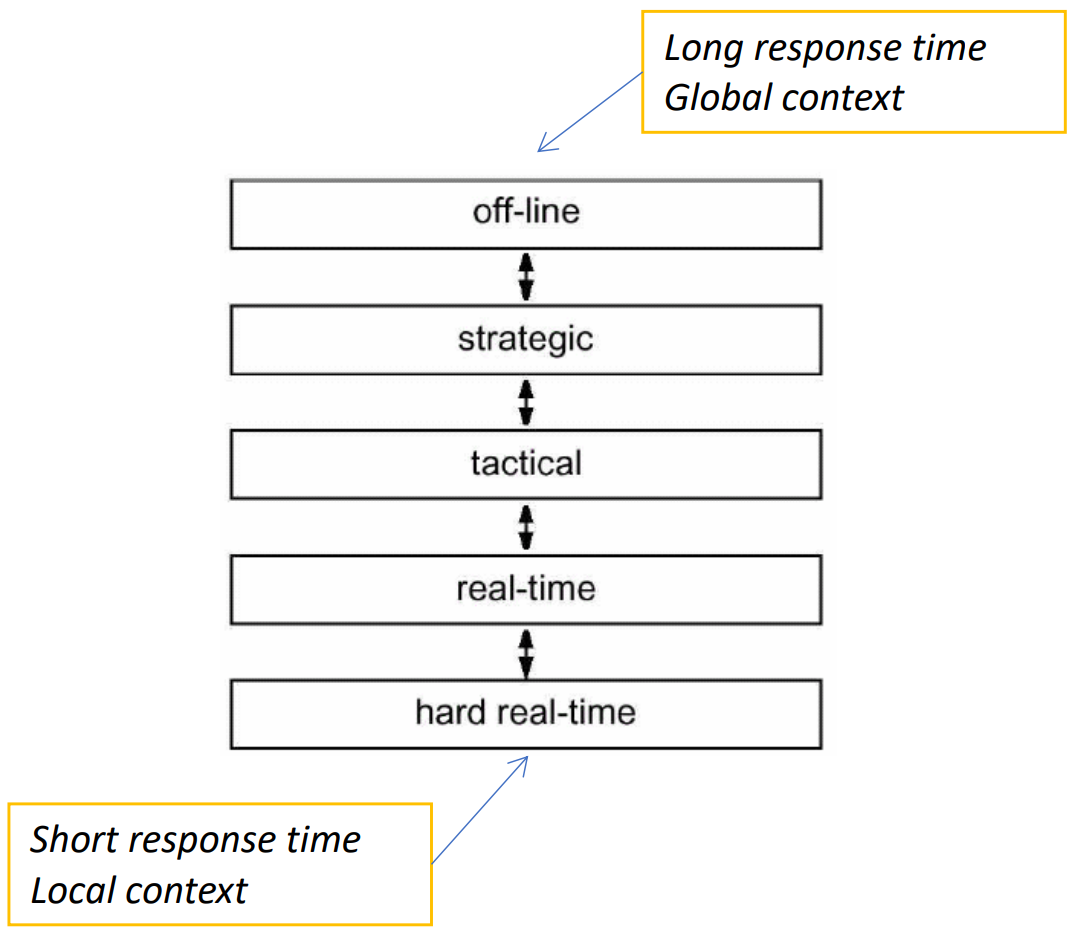
\includegraphics[width=0.35\linewidth]{figures/temporal_decomp}
	\end{center}
	\caption{Types of time demands for \textit{temporal decomposition}.}
	\label{fig:temporal_decomp}
\end{figure}

\subsection{What is ROS?}%

\subsubsection{ROS Nodes}%

Typically, we try to divide software into different modules, each of which performs a specific task. In ROS, these
modules are run over a single or multiple \textit{Nodes}.

\begin{defn}{Node}
	a process that performs some computation.
\end{defn}

Nodes are combined together into a graph and communicat with each other using streaming \textit{topics}. Nodes
\textbf{do not} communicate with each other directly, otherwise we can get into the craziness and complications of the
other architectures discussed above.

\subsubsection{ROS Topics}%

\begin{defn}{Topic}
	a named bus over which nodes exchange messages
\end{defn}

\begin{itemize}
	\item Topics have \textbf{anonymous} publish/subscribe semantics, i.e. no one knows who published a message or read
	a message
	\item Can be \textit{multiple} publisher and subscribers to a topic
	\item Strongly typed
\end{itemize}

\subsubsection{ROS Messages}%
\begin{defn}{Message}
	a simple data structure comprising strongly typed fields which is used for one node to communicate to other nodes
\end{defn}

\section{Locomotion}%
\begin{defn}{Locomotion}
	enabling a robot to move
\end{defn}

\hfill\\

\noindent
Wheeled locomotion is simple, safe, and stable. Key issues for wheeled locomotion include
\begin{itemize}
	\item Stability
	\begin{itemize}
		\item Number and geometry of contact points
		\item Centre of gravity
		\item Static/dynamic stability
		\item Inclination of terrain
	\end{itemize}
	\item Characteristics of contact
	\begin{itemize}
		\item Contact point/path size and shape
		\item Angle of contact
		\item Friction
	\end{itemize}
	\item Type of environment
\end{itemize}

\hfill

\noindent
\textbf{Legged mobile robots} can adapt to human terrain, but they have lots of limitations: power and mechanical complexity,
high degrees of freedom, control system complexity, etc.

\subsection{Leg Locomotion}%
\noindent
\textbf{Degree of Freedom} (DOF): joints or axes in motion

\hfill

\noindent
A minimum of two DOFs is required to move a leg forward, but usually legs have three degrees of freedom. A fourth DOF is
needed for the angle joint, which might improve walking.

\hfill

\noindent
As you add more DOFs, the complexity of the system increases very fast.

\hfill

\noindent
Arms need 6 or 7 DOFs.

\hfill

\noindent
\textit{Often, clever mechanical design can perform the same operations as complex active control circuitry.}

\hfill \\ \hfill \\

\hfill \textbf{Thu 12 Jan 2023}

\noindent
\textbf{Gait control}: how legs are coordinated for movement, e.g. crawl, trot, pace, bound, pronk, gallop, etc.

\hfill \\
\noindent
Number of gaits is $(2k - 1)!$ where $k$ is the number of legs.

\hfill \\
\noindent
\textbf{Cost of transportation}:
\begin{itemize}
	\item How much energy a robot uses to travel a certain distance
	\item Usually normalized by the robot weight
	\item Measured in $\frac{J}{N-m}$
	\item Driving on wheels has very low cost of transportation.
\end{itemize}

\hfill \\
\noindent
Legged robot control should be designed to better exploit the dynamics of the system. For example passive dynamic
walking.

\subsection{Wheeled Mobile Robots}%
\noindent
Wheels are \textit{the most popular locomotion mechanisms}:
\begin{itemize}
	\item Highly efficient
	\item Simple mechanical implementation
	\item Balancing is not \textit{usually} a problem, but a suspension system is needed to allow all wheel to maintain
		ground contact on uneven terrain.
\end{itemize}

\hfill \\
\noindent
We will focus on:
\begin{itemize}
	\item Traction
	\item Stability
	\item Maneuverability
	\item Control -- we will mostly focus on this
\end{itemize}

\hfill \\
\noindent
Wheel Designs:
\begin{itemize}
	\item Standard wheels
	\begin{itemize}
		\item 2 DOFs
	\end{itemize}
	\item Castor wheels
	\begin{itemize}
		\item 2 DOFs
		\item Can move while the contact point of the wheel stays the same.
		\item If something is super heavy, it's easier to get momentum with these wheels
		\item Harder to control
	\end{itemize}
	\item Swedish (Omni) wheels
	\begin{itemize}
		\item 3 DOFs
	\end{itemize}
	\item Ball or spherical wheel
	\begin{itemize}
		\item 3 DOFs
		\item Balled computer mice used these
		\item Suspension issue -- hard to get suspension on these
	\end{itemize}
\end{itemize}

\hfill \\
\noindent
Stability of a vehicle is guaranteed with 3 wheels -- centre of gravity is required to be within the triangle formed by
ground contact points of wheels.

\hfill\\
\noindent
Stability is improved by 4 and more wheels

\hfill \\
\noindent
\begin{defn}{Holonomic}
	refers to the relationship between controllable and total degrees of freedom of a robot. If the controllable degrees
	of freedom is equal to the total degrees of freedom, then the robot is said to be \textbf{holonomic}. If a robot is
	holonomic, it can move in any direction in its configuraiton space.
\end{defn}

\hfill \\
\noindent
Combining \textbf{actuation} and \textbf{steering} on one wheel makes design complex and adds additional errors for
odometry.

\hfill \\
\noindent
Static stability with two wheels can be achieved by \textbf{ensuring centre of mass is below the wheel axis} or by using
fancy controllers.

\subsection{Motion Control}%
\begin{itemize}
	\item Kinematic/dynamic model of the robot comes in here
	\item Model the interaction between the wheel and ground
	\item Definition of required motion -- which motion is required:
	\begin{itemize}
		\item Speed control
		\item Position control
	\end{itemize}
	\item Control law that satisfies the requirements
\end{itemize}

\hfill \\
\noindent
\textbf{Kinematics}: Description of mechanical behaviour of the robot for design and control. E.g. hwo a robot will move
given motor inputs.

\hfill \\
\noindent
\textbf{Mobile robots} can move unbounded with respect to their environment:
\begin{itemize}
	\item No direct way to measure robot's position
	\item Position must be integrated over time
	\item Leads to inaccuracies of the position (motion) estimate
\end{itemize}

\hfill \\
\noindent
\begin{defn}{Configuration}
	a complete specification of the position of every point of the robotic system (position and orientation). This is
	sometimes also called a \textbf{pose}.
\end{defn}

\begin{defn}{Configuration Space}
	The space of all possible configurations, which can be thought of as one of the robot's frame of references.
\end{defn}

\begin{figure}
	\centering
	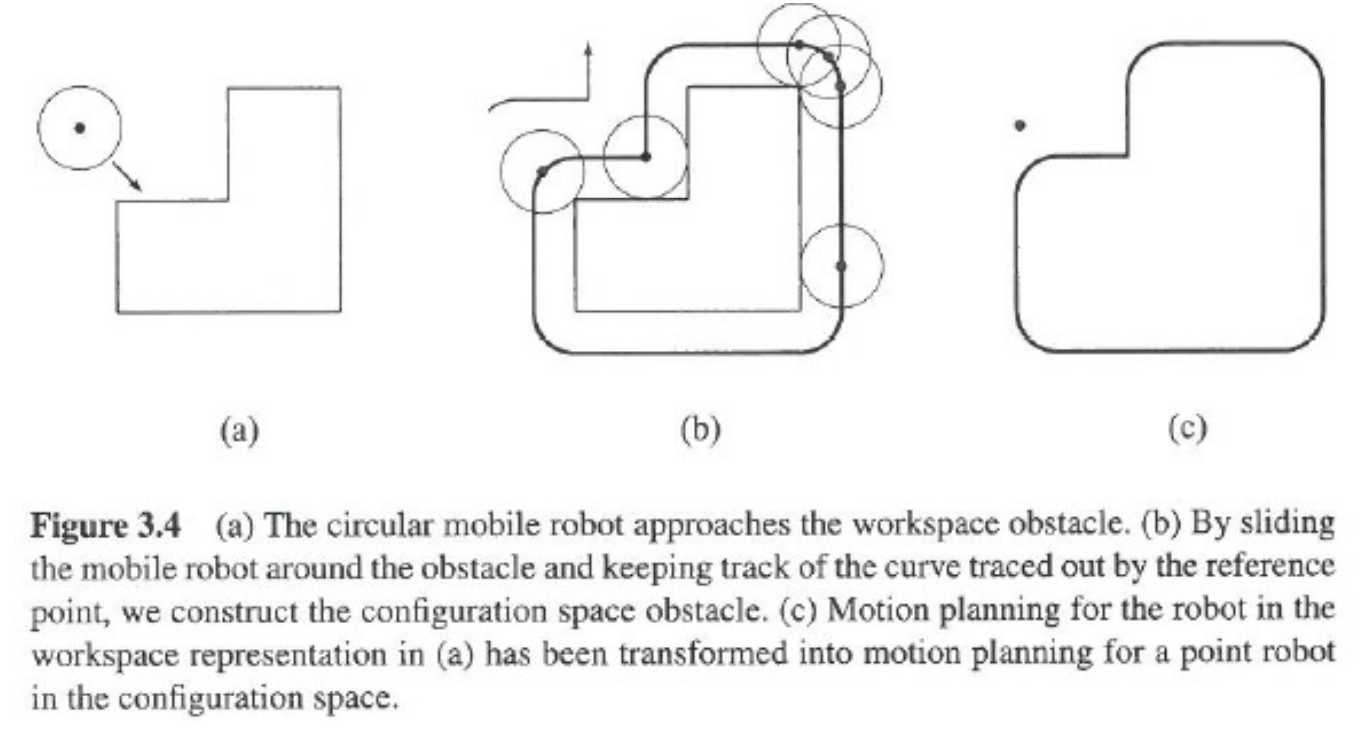
\includegraphics[width=\linewidth]{figures/cspace}
	\caption{(a)A circular mobile in the workspace. The configuration space is the set of all points in space that the
	robot can be in. By re-representing the circular robot as a point, we can (b) adjust the workspace to result in the
	same configuration space and (c) consider the robot as a single point which simplifies calculations.}
	\label{fig:config_space}
\end{figure}

\begin{figure}
	\centering
	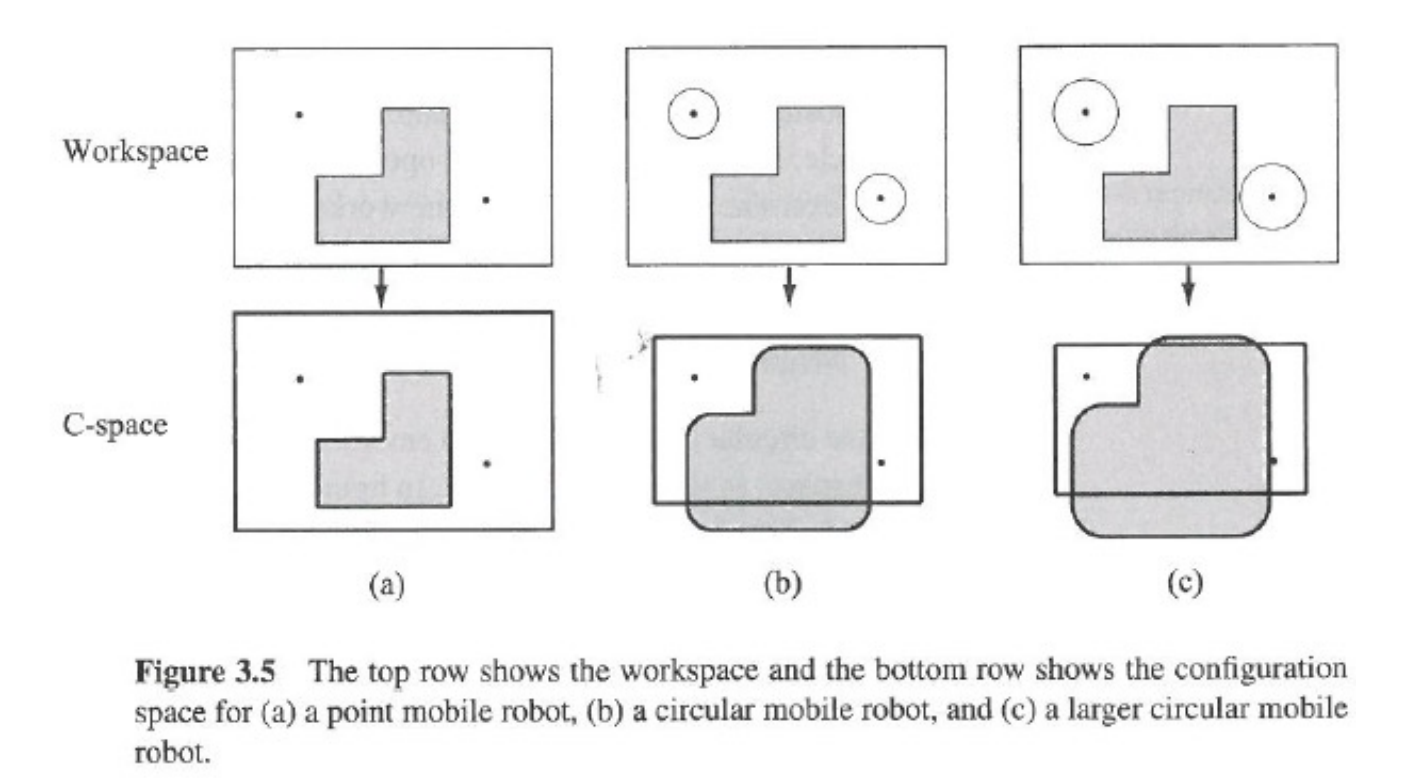
\includegraphics[width=\linewidth]{figures/cspace2}
\end{figure}

\begin{defn}{Workspace}
	the 2D or 3D \textbf{ambient} space the robot is in
\end{defn}

\section{Kinematics}%
\begin{defn}{Kinematics}
	computing how a robot will move given motor inputs
\end{defn}

\begin{defn}{Inverse Kinematics}
	computing how to move motors to get a robot to do what we want
\end{defn}

\hfill \\
\noindent
There are two frames that we need to worry about:
\begin{itemize}
	\item \textbf{Initial frame}: the world - $\xi_{i} = (x_{i}, y_{i}, \theta_{i})$
	\item \textbf{Robot frame}: think of yourself as the robot - $\xi_{r} = (x_{r}, y_{r}, \theta_{r})$
\end{itemize}

\hfill \\
\noindent
Robot is at initial frame $\xi_{i} = (x_{i}, y_{i}, \theta_{i})$. We want to get to some location, but we can't control $(x_i,
y_{i}, \theta_{i})$ directly. Instead, the robot can only control $\xi_{r}$.

\hfill \\ \noindent Consider a wheeled robot where the robot can know the speed of wheel $i$: $\dot \phi_{i} \forall i =
1, \ldots, n$, steering angle of steerable wheel $j$: $\beta_{j} \forall j = 1, \ldots, m$, and speed with which
steering angle for wheel $j$ is changing: $\dot \beta_{j}$. These define the forward motion of the robot or the
\textit{forward kinematics}.

\hfill \\
\noindent
In the robot frame, we have $\xi_{r} = (x_{r}, y_{r}, \theta_{r})$. But, since a wheeled robot is always facing straight
forward, we have $\theta_{r} = 0$. We will simply re-define $\theta_{r} = \theta_{i}$. We have the forward kinematics
to be: \[
	f(\dot \phi_{i}, \ldots, \dot \phi_{n}, \beta_{1}, \ldots, \beta_{m}, \dot \beta_{1}, \ldots, \dot \beta_{m}) =
	[\dot x_{i} \quad \dot y_{i} \quad \dot \theta_{i} ]^{\top}
.\]
Inverse kinematics would give us: \[
	[\dot \phi_{i} \ \ldots \ \dot \phi_{n} \ \beta_{1} \ \ldots \ \beta_{m} \ \dot \beta_{1} \ \ldots \ \dot \beta_{m}]^{\top} =
	f^{-1}(\dot x_{i}, \dot y_{i}, \dot \theta_{i})
.\]

\hfill \\
\noindent
What we want to do now is:
\begin{equation}
	\dot \xi_{r} = \begin{pmatrix} \dot x_{r} \\ \dot y_{r} \\ \dot \theta_{r} \end{pmatrix} =
	\bm{R}_{\theta} \begin{pmatrix} \dot x_{i} \\ \dot y_{i} \\ \dot \theta_{i} \end{pmatrix} = \bm{R}_{\theta} \dot
	\xi_{i}\qquad \text{where }
	\bm{R}_{\theta} = \begin{pmatrix} \cos(\theta) & \sin(\theta) & 0 \\ - \sin(\theta) & \cos(\theta) & 0 \\ 0 & 0 & 1 \end{pmatrix}
\end{equation}
where $\theta = \theta_{i} = \theta_{r}$. We get
\begin{align}
	\dot x_{r} &= \dot x_{i} \cos(\theta) + \dot y_{i} \sin(\theta) \\
	\dot y_{r} &= - \dot x_{i} \sin(\theta) + \dot y_{i} \cos(\theta) \\
	\dot \theta_{r} &= \dot \theta_{i}
\end{align}

\hfill \\
\noindent
Still, this isn't what we want, we want the inverse-kinematics, not the kinematics:
\begin{equation}
	\begin{pmatrix} \dot x_{i} \\ \dot y_{i} \\ \dot \theta_{i} \end{pmatrix} =
	\bm{R}_{\theta}^{-1} \begin{pmatrix} \dot x_{r} \\ \dot y_{r} \\ \dot \theta_{r} \end{pmatrix} \qquad
	\text{where }
	\bm{R}_{\theta}^{-1} = \begin{pmatrix} \cos(\theta) & -\sin(\theta) & 0 \\ \sin(\theta) & \cos(\theta) & 0 \\ 0 & 0 & 1 \end{pmatrix}
\end{equation}
this tells us how to change the robot's wheels to get somewhere in the world. In our case, $\dot y_{r} = 0$ always:
\begin{align}
	\dot x_{i} &= \dot x_{r} \cos(\theta) - \dot y_{r} \sin(\theta) \\
	\dot y_{i} &= \dot x_{r} \sin(\theta) + \dot y_{r} \cos(\theta) \\
	\dot \theta_{i} &=  \dot \theta_{r}
\end{align}

\hfill \\ \noindent So, if we know the relative changes in $x$, $y$, and $\theta$, we can find the global position. How
do we know what these values are?


\hfill \\
\noindent
Constraints and assumptions:
\begin{itemize}
	\item Movement on a horizontal plane
	\item Point contact of wheels
	\item Wheels are not deformable
	\item Pure rolling: velocity is 0 at contact point
	\item ...
\end{itemize}

\hfill \\
\noindent
Differential Drive:
\begin{itemize}
	\item The \textbf{differential drive} is a two-wheeled drive system with independent actuators for each wheel. The name
		refers to the fact that the motion vector of the robot is the sum of the independent wheel motions, and so
		turning can be accomplished by rotating the wheels at different speeds. The drive
		wheels are usually placed on each side of the robot and toward the front.
	\item Wheels rotate at $\dot \phi$
	\item Each wheel contributes $\frac{r \dot \phi}{2}$ to the motion of centre of rotation.
	\item Speed: sum of two wheels
	\item Rotation: due to the right wheel is $\omega_{r} = \frac{r \dot \phi}{2 l}$ counterclockwise about left wheel,
		where $l$ is the distance between the wheel and centre of rotation.
	\item Combining components
	\begin{equation}
		\begin{pmatrix} \dot x_{r} \\ \dot y_{r} \\ \dot \theta_{r} \end{pmatrix}  = \begin{pmatrix} \frac{r \dot
	\phi_{r}}{2} + \frac{r \dot \phi_{l}}{2} \\ 0 \\ \frac{r\dot \phi_{r}}{2l} - \frac{r\dot \phi_{l}}{2l} \end{pmatrix}
	\end{equation}
\end{itemize}
now, what is the change in the initial frame of reference?


\hfill

\hfill \textbf{Tue 17 Jan 2023} \\

\noindent
Kinematics works in a perfect world, with all our above assumptions satisfied, and where the robot is a point mass. In
this case, opened-loop controllers like kinematics work.

\hfill \\

\noindent
Sliding constraint:
\begin{itemize}
	\item Standard wheel has no lateral motion, we can have steered standard wheels or steered caster wheels
	\item Move in circle whose centre is on \textit{zero motion line} through the axis
\end{itemize}

\hfill

\noindent
\textbf{Degree of Mobility}: number of degrees of freedom of robot chassis that can be immediately manipulated through
changes in wheel velocity.

\hfill

\noindent
\textbf{Degree of Maneuverability}: the overall degrees of freedom that a robot can manipulate: $\delta_{M} = \delta_{m}
+ \delta_{s}$

\hfill

\noindent
We may want a robot to be \textbf{redundant} if it needs to get to a certain point. If one path is blocked, it can take
another path e.g. Think of a manipulator attempting to get its end effector to a certain position. If one trajectory is
blocked, it can make another.

\section{Manipulators}%

A \textbf{manipulator} is some robot that manipulates (physically alters) something in the real world, but not its own
position, at least as a primary goal. Desirable in dangerous, dirty, or dull workspaces.

\hfill

\hfill \textbf{Thu 19 Jan 2023}

\hfill

\noindent
\textbf{Actuator}: generates motion or force, usually a motor

\hfill \\
\noindent
For wheels on a robot, we want them synchronized so we typically want to use a servo motor and not a DC motor.

\hfill \\
\noindent


\end{document}
